\clearpage

\section{IQ Modulator}

\begin{tcolorbox}	
	\begin{tabular}{p{2.75cm} p{0.2cm} p{10.5cm}} 	
		\textbf{Header File}   &:& iq\_modulator.h \\
		\textbf{Source File}   &:& iq\_modulator.cpp \\
	\end{tabular}
\end{tcolorbox}

This blocks accepts one inupt signal continuous in both time and amplitude and it can produce either one or two output signals. It generates an optical signal and it can also generate a binary signal.

\subsection*{Input Parameters}

\begin{table}[h]
	\centering
	\begin{tabular}{|c|c|c|c|cccc}
		\cline{1-4}
		\textbf{Parameter} & \textbf{Type} & \textbf{Values} &   \textbf{Default}& \\ \cline{1-4}
		outputOpticalPower & double & any & $1e-3$ \\ \cline{1-4}
		outputOpticalWavelength & double & any & $1550e-9$ \\ \cline{1-4}
		outputOpticalFrequency & double & any & speed\_of\_light/outputOpticalWavelength \\ \cline{1-4}
	\end{tabular}
	\caption{Binary source input parameters}
	\label{table:iqmod_in_par}
\end{table}

%\begin{itemize}
%	\item outputOpticalPower\{1e-3\} \linebreak
%	(double)
%	\item outputOpticalWavelength\{1550e-9\} \linebreak (double)
%	\item outputOpticalFrequency\{speed$\_$of$\_$light/outputOpticalWavelength\} \linebreak
%	(double)
%\end{itemize}

\subsection*{Methods}

IqModulator(vector$<$Signal *$>$ \&InputSig, vector$<$Signal *$>$ \&OutputSig) :Block(InputSig, OutputSig)\{\};
\bigbreak
void initialize(void);
\bigbreak
bool runBlock(void);
\bigbreak
void setOutputOpticalPower(double outOpticalPower)
\bigbreak
void setOutputOpticalPower$\_$dBm(double outOpticalPower$\_$dBm)
\bigbreak
void setOutputOpticalWavelength(double outOpticalWavelength)
\bigbreak
void setOutputOpticalFrequency(double outOpticalFrequency)

\subsection*{Functional Description}

This block takes the two parts of the signal: in phase and in amplitude and it combines them to produce a complex signal that contains information about the amplitude and the phase.

This complex signal is multiplied by $\frac{1}{2}\sqrt{\textit{outputOpticalPower}}$ in order to reintroduce the information about the energy (or power) of the signal. This signal corresponds to an optical signal and it can be a scalar or have two polarizations along perpendicular axis. It is the signal that is transmited to the receptor.

The binary signal is sent to the Bit Error Rate (BER) meaurement block.

\subsection*{Input Signals}

\subparagraph*{Number}: 2

\subparagraph*{Type}: Sequence of impulses modulated by the filter (ContinuousTimeContiousAmplitude))

\subsection*{Output Signals}

\subparagraph*{Number}: 1 or 2

\subparagraph*{Type}: Complex signal (optical) (ContinuousTimeContinuousAmplitude) and binary signal (DiscreteTimeDiscreteAmplitude)

\subsection*{Example}
\begin{figure}[h]
	\centering
	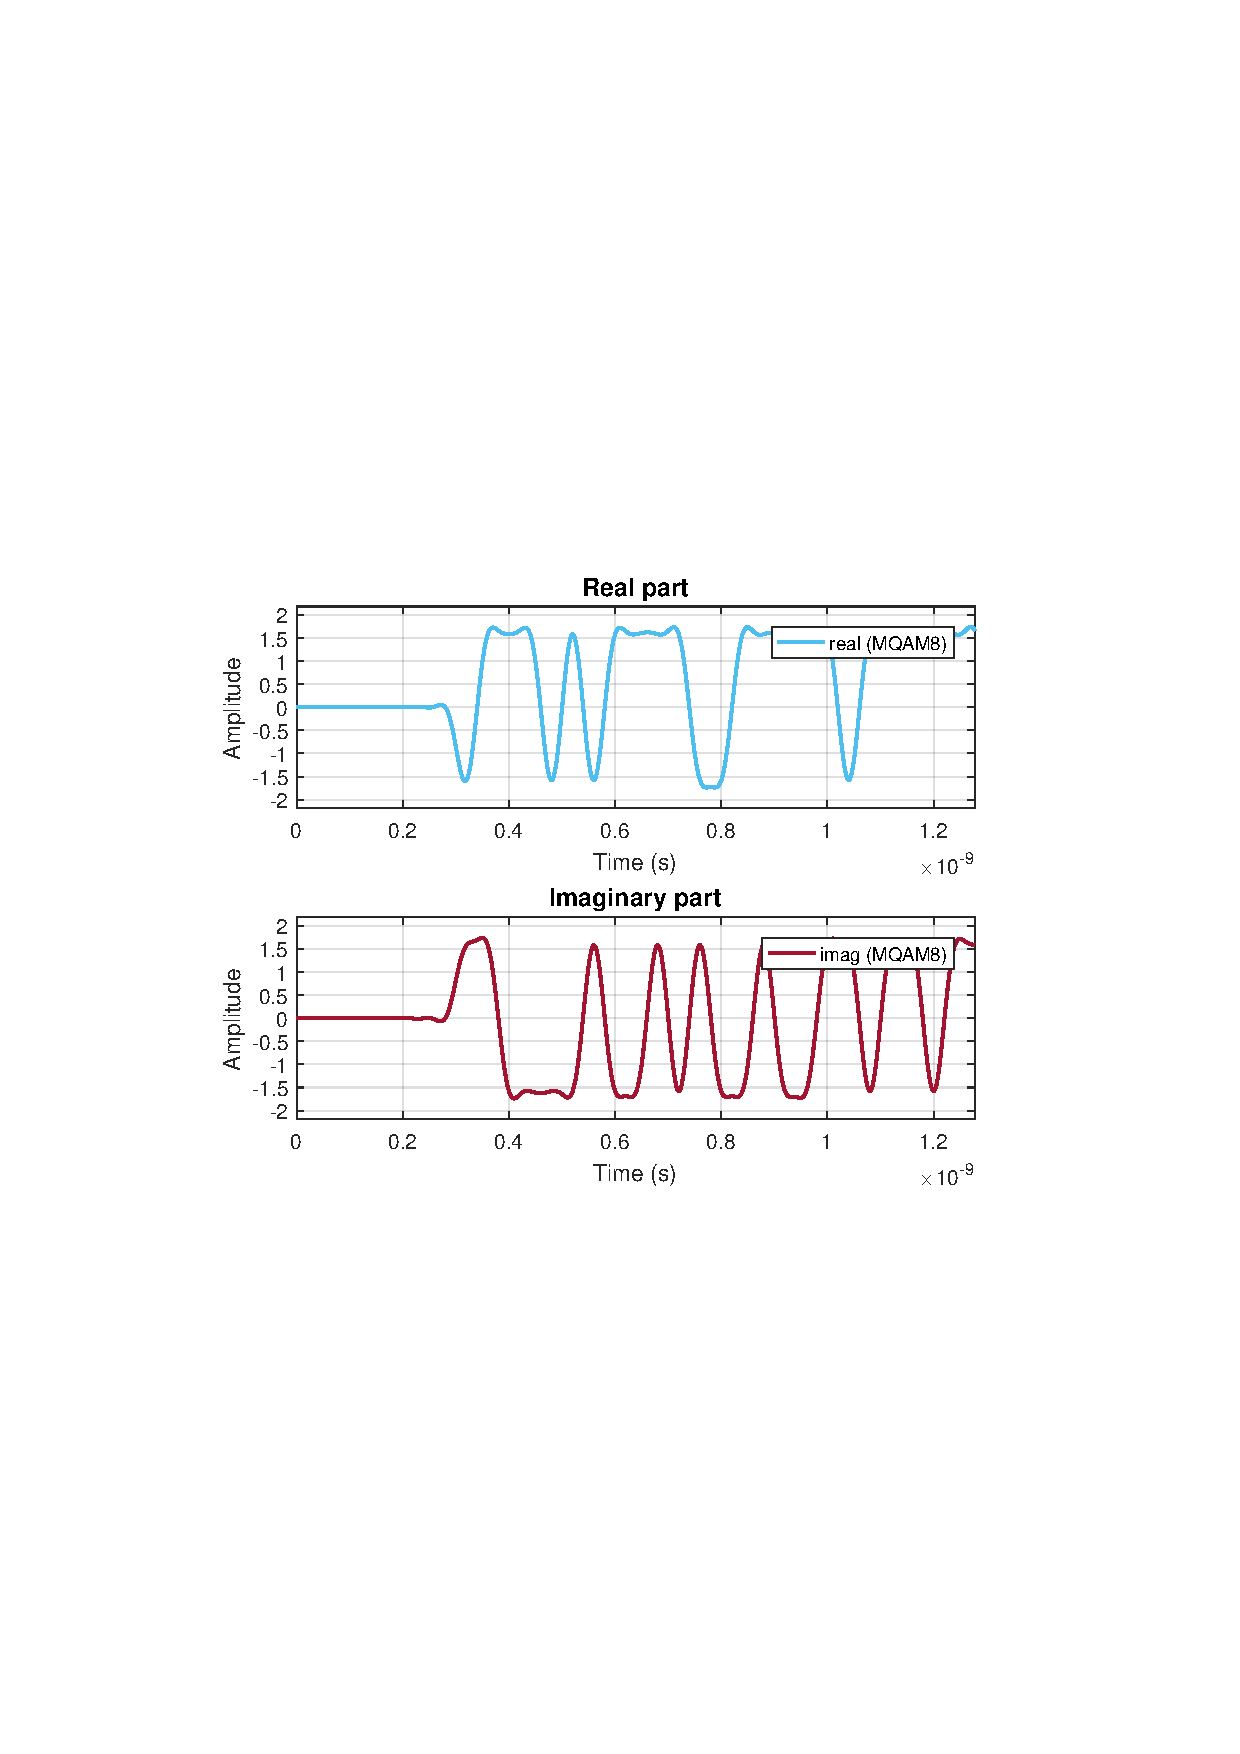
\includegraphics[clip, trim=0.5cm 9cm 0.5cm 9cm, width=\textwidth]{./lib/iq_modulator/figures/MQAM_iq_modulator_output.pdf}
	\label{MQAM8_DeterministicAppendZeros}\caption{Example of a signal generated by this block for the initial binary signal 0100...}
\end{figure}

%\subsection*{Sugestions for future improvement}
